{[}\href{quickstart.html}{Previous: Installing and Running Terrier}{]}
{[}\href{index.html}{Contents}{]} {[}\href{configure_general.html}{Next:
Configuring Terrier}{]}

\section{Terrier Components}\label{terrier-components}

On this page we will give an overview of Terrier's main components and
their interaction.

\subsection{Component Interaction}\label{component-interaction}

\subsubsection{Indexing}\label{indexing}

The graphic below gives an overview of the interaction between the main
components involved in the indexing process.

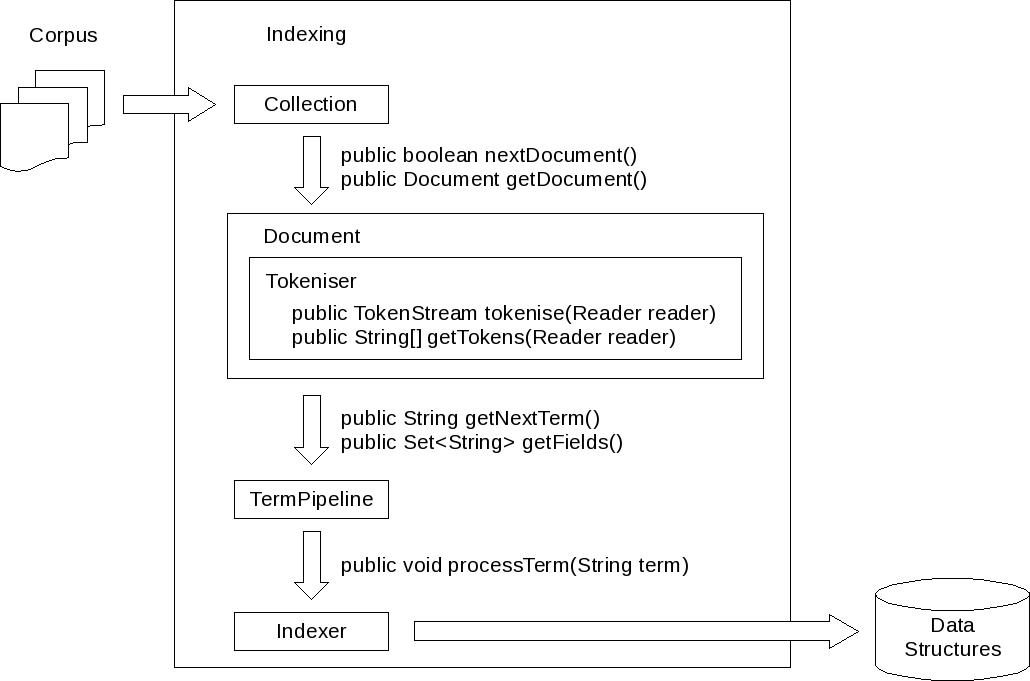
\includegraphics[width=0.66000\textwidth]{images/indexing_architecture.png}

\begin{itemize}
\tightlist
\item
  A corpus will be represented in the form of a
  \href{javadoc/org/terrier/indexing/Collection.html}{Collection}
  object. Raw text data will be represented in the form of a
  \href{javadoc/org/terrier/indexing/Document.html}{Document} object.
  Document implementations usually are provided with an instance of a
  \href{javadoc/org/terrier/indexing/tokenisation/Tokeniser.html}{Tokeniser}
  class that breaks pieces of text into single indexing tokens.
\item
  The indexer is responsible for managing the indexing process. It
  iterates over the documents of the collection and sends each term
  found through a
  \href{javadoc/org/terrier/terms/TermPipeline.html}{TermPipeline}
  component.
\item
  A TermPipeline can transform terms or remove terms that should not be
  indexed. An example for a TermPipeline chain is
  \texttt{termpipelines=Stopwords,PorterStemmer}, which removes terms
  from the document using the
  \href{javadoc/org/terrier/terms/Stopwords.html}{Stopwords} object, and
  then applies Porter's Stemming algorithm for English to the terms
  (\href{javadoc/org/terrier/terms/PorterStemmer.html}{PorterStemmer}).
\item
  Once terms have been processed through the TermPipeline, they are
  aggregated and the following data structures are created by their
  corresponding DocumentBuilders: DirectIndex, DocumentIndex, Lexicon,
  and InvertedIndex.
\item
  For single-pass indexing, the structures are written in a different
  order. Inverted file postings are built in memory, and committed to
  `runs' when memory is exhausted. Once the collection had been indexed,
  all runs are merged form the inverted index and the lexicon.
\end{itemize}

\subsection{Retrieval}\label{retrieval}

The graphic below gives an overview of the interaction of Terrier's
components in the retrieval phase.

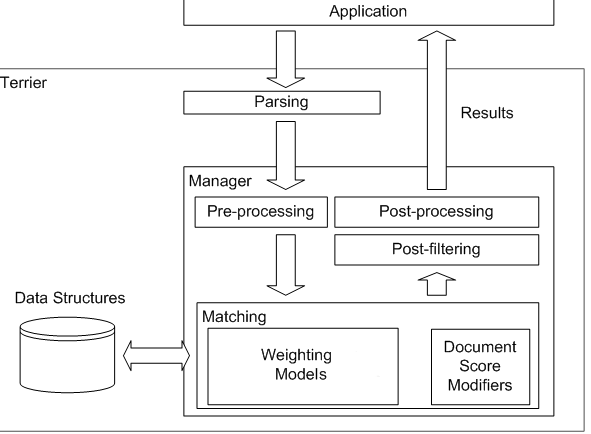
\includegraphics{images/retrieval_architecture.png}

\begin{itemize}
\tightlist
\item
  An application, such as for example the Desktop Terrier or TrecTerrier
  applications, issues a query to the Terrier framework.
\item
  In a first step the query will be parsed and an instantiation of a
  Query object will take place.
\item
  Afterwards, the query will be handed to the Manager component. The
  manager firstly pre-processes the query, by applying it to the
  configured TermPipeline.
\item
  After the Pre-Processing the query will be handed to the Matching
  component. The Matching component is responsible for initialising the
  appropriate WeightingModel and DocumentScoreModifiers. Once all these
  components have been instantiated, the computation of document scores
  with respect to the query will take place.
\item
  Afterwards, the PostProcessing and PostFiltering takes place. In
  PostProcessing, the ResultSet can be altered in any way - for example,
  QueryExpansion expands the query, and then calls Matching again to
  generate an improved ranking of documents. PostFiltering is simpler,
  allowing documents to be either included or excluded - this is ideal
  for interactive applications where users want to restrict the domain
  of the documents being retrieved.
\item
  Finally, the ResultSet will be returned to the application component.
\end{itemize}

\subsection{Component description}\label{component-description}

Here we provide a listing and brief description of Terrier's components.

\subsubsection{Indexing}\label{indexing-1}

\begin{longtable}[]{@{}ll@{}}
\toprule
\textbf{Name} & \textbf{Description}\tabularnewline
\midrule
\endhead
\textbf{Collection} & This component encapsulates the most fundamental
concept to indexing with Terrier - a Collection i.e. a set of documents.
See
\href{javadoc/org/terrier/indexing/Collection.html}{org.terrier.indexing.Collection}
for more details.\tabularnewline
\textbf{Document} & This component encapsulates the concept of a
document. It is essentially an Iterator over terms in a document. See
\href{javadoc/org/terrier/indexing/Document.html}{org.terrier.indexing.Document}
for more details.\tabularnewline
\textbf{Tokeniser} & Used by Document objects to break sequences of text
(e.g. sentences) into a stream of words to index. See
\href{javadoc/org/terrier/indexing/tokenisation/Tokeniser.html}{org.terrier.indexing.tokenisation.Tokeniser}
for more details.\tabularnewline
\textbf{TermPipeline} & Models the concept of a component in a pipeline
of term processors. Classes that implement this interface could be
stemming algorithms, stopwords removers, or acronym expansion just to
mention few examples. See
\href{javadoc/org/terrier/terms/TermPipeline.html}{org.terrier.terms.TermPipeline}
for more details.\tabularnewline
\textbf{Indexer} & The component responsible for managing the indexing
process. It instantiates TermPipelines and Builders. See
\href{javadoc/org/terrier/structures/indexing/Indexer.html}{org.terrier.structures.indexing.Indexer}
for more details.\tabularnewline
\textbf{Builders} & Builders are responsible for writing an index to
disk. See
\href{javadoc/org/terrier/structures/indexing/package-summary.html}{org.terrier.structures.indexing
package} for more details.\tabularnewline
\bottomrule
\end{longtable}

\subsubsection{Data Structures}\label{data-structures}

\begin{longtable}[]{@{}ll@{}}
\toprule
\textbf{Name} & \textbf{Description}\tabularnewline
\midrule
\endhead
\textbf{BitFile} & A highly compressed I/O layer using gamma and unary
encodings. See the org.terrier.compression packages for more
details.\tabularnewline
\textbf{Direct Index} & The direct index stores the identifiers of terms
that appear in each document and the corresponding frequencies. It is
used for automatic query expansion, but can also be used for user
profiling activities. See
\href{javadoc/org/terrier/structures/bit/DirectIndex.html}{org.terrier.structures.bit.DirectIndex}
for more details.\tabularnewline
\textbf{Document Index} & The document index stores information about
each document for example the document length and identifier, and a
pointer to the corresponding entry in the direct index. See
\href{javadoc/org/terrier/structures/DocumentIndex.html}{org.terrier.structures.DocumentIndex}
for more details.\tabularnewline
\textbf{Inverted Index} & The inverted index stores the posting lists,
i.e. the identifiers of the documents and their corresponding term
frequencies. Moreover it is capable of storing the position of terms
within a document. See
\href{javadoc/org/terrier/structures/bit/InvertedIndex.html}{org.terrier.structures.bit.InvertedIndex}
for more details.\tabularnewline
\textbf{Lexicon} & The lexicon stores the collection vocabulary and the
corresponding document and term frequencies. See
\href{javadoc/org/terrier/structures/Lexicon.html}{org.terrier.structures.Lexicon}
for more details.\tabularnewline
\textbf{Meta Index} & The Meta Index stores additional (meta)
information about each document, for example its unique textual
identifier (docno) or URL. See
\href{javadoc/org/terrier/structures/MetaIndex.html}{org.terrier.structures.MetaIndex}
for more details.\tabularnewline
\bottomrule
\end{longtable}

\subsubsection{Retrieval}\label{retrieval-1}

\textbf{Name}

\textbf{Description}

\textbf{Manager}

This component is responsible for handling/coordinating the main
high-level operations of a query. These are:

\begin{itemize}
\tightlist
\item
  Pre Processing (Term Pipeline, Control finding, term aggregation)
\item
  Matching
\item
  Post-processing
\item
  Post-filtering
\end{itemize}

See
\href{javadoc/org/terrier/querying/Manager.html}{org.terrier.querying.Manager}
for more details.

\textbf{Matching}

The matching component is responsible for determining which documents
match a specific query and for scoring documents with respect to a
query. See
\href{javadoc/org/terrier/matching/Matching.html}{org.terrier.matching.Matching}
for more details.

\textbf{Query}

The query component models a query, that consists of sub-queries and
query terms. See
\href{javadoc/org/terrier/querying/parser/Query.html}{org.terrier.querying.parser.Query}
for more details.

\textbf{Weighting Model}

The Weighting model represents the retrieval model that is used to
weight the terms of a document. See
\href{javadoc/org/terrier/matching/models/WeightingModel.html}{org.terrier.matching.models.WeightingModel}
for more details.

\textbf{Document Score Modifiers}

Responsible for query dependent modification document scores. See
\href{javadoc/org/terrier/matching/dsms/package-summary.html}{org.terrier.matching.dsms
package} for more details.

\subsubsection{Applications}\label{applications}

\begin{longtable}[]{@{}ll@{}}
\toprule
\textbf{Name} & \textbf{Description}\tabularnewline
\midrule
\endhead
\textbf{Trec Terrier} & An application that enables indexing and
querying of TREC collections. See
\href{javadoc/org/terrier/applications/TrecTerrier.html}{org.terrier.applications.TrecTerrier}
for more details.\tabularnewline
\textbf{Desktop Terrier} & An application that allows for indexing and
retrieval of local user content. See
\href{javadoc/org/terrier/applications/desktop/package-summary.html}{org.terrier.applications.desktop
package} for more details.\tabularnewline
\textbf{HTTP Terrier} & An application that allows for retrieval of
documents from a browser. See src/webapps/results.jsp for more details,
or the \href{terrier_http.html}{relevant documentation}.\tabularnewline
\bottomrule
\end{longtable}

{[}\href{quickstart.html}{Previous: Installing and Running Terrier}{]}
{[}\href{index.html}{Contents}{]} {[}\href{configure_general.html}{Next:
Configuring Terrier}{]}

\begin{center}\rule{0.5\linewidth}{\linethickness}\end{center}

Webpage: \url{http://terrier.org}\\
Contact:
\href{mailto:terrier@dcs.gla.ac.uk}{\nolinkurl{terrier@dcs.gla.ac.uk}}\\
\href{http://www.dcs.gla.ac.uk/}{School of Computing Science}\\
Copyright (C) 2004-2015 \href{http://www.gla.ac.uk/}{University of
Glasgow}. All Rights Reserved.
